\documentclass[conference]{IEEEtran}
\IEEEoverridecommandlockouts
% The preceding line is only needed to identify funding in the first footnote. If that is unneeded, please comment it out.
%Template version as of 6/27/2024

\usepackage{graphicx}
\usepackage{dblfloatfix} % fixes figure* placement issues
\usepackage{cite}
\usepackage{amsmath,amssymb,amsfonts}
\usepackage{algorithmic}
\usepackage{textcomp}
\usepackage{xcolor}
\usepackage{placeins}
\def\BibTeX{{\rm B\kern-.05em{\sc i\kern-.025em b}\kern-.08em
    T\kern-.1667em\lower.7ex\hbox{E}\kern-.125emX}}
\begin{document}

\title{Multi-Agent Reasoning System for IPC Cases}

\author{\IEEEauthorblockN{1\textsuperscript{st} Given Name Surname}
\IEEEauthorblockA{\textit{dept. name of organization (of Aff.)} \\
\textit{name of organization (of Aff.)}\\
City, Country \\
email address or ORCID}
\and
\IEEEauthorblockN{2\textsuperscript{nd} Given Name Surname}
\IEEEauthorblockA{\textit{dept. name of organization (of Aff.)} \\
\textit{name of organization (of Aff.)}\\
City, Country \\
email address or ORCID}
\and
\IEEEauthorblockN{3\textsuperscript{rd} Given Name Surname}
\IEEEauthorblockA{\textit{dept. name of organization (of Aff.)} \\
\textit{name of organization (of Aff.)}\\
City, Country \\
email address or ORCID}
\and
\IEEEauthorblockN{4\textsuperscript{th} Given Name Surname}
\IEEEauthorblockA{\textit{dept. name of organization (of Aff.)} \\
\textit{name of organization (of Aff.)}\\
City, Country \\
email address or ORCID}
\and
\IEEEauthorblockN{5\textsuperscript{th} Given Name Surname}
\IEEEauthorblockA{\textit{dept. name of organization (of Aff.)} \\
\textit{name of organization (of Aff.)}\\
City, Country \\
email address or ORCID}
\and
\IEEEauthorblockN{6\textsuperscript{th} Given Name Surname}
\IEEEauthorblockA{\textit{dept. name of organization (of Aff.)} \\
\textit{name of organization (of Aff.)}\\
City, Country \\
email address or ORCID}
}

\maketitle

\begin{abstract}
Indian Penal Code (IPC) case analysis requires combining statutory interpretation, precedent grounding, and adversarial reasoning. Single-pass large language model outputs are often fluent but inconsistent, weakly grounded, and difficult to audit in legal settings. We present a multi-agent retrieval-augmented generation system for IPC case reasoning with three specialized agents: prosecutor, defence, and judge. The prosecutor and defence agents retrieve supporting statutes and precedents, while the judge is explicitly constrained to reason only over evidence surfaced by both sides, preventing additional hidden retrieval at adjudication time. The system uses a hybrid FAISS + BM25 retriever for statutes and precedent cases, structured preprocessing for legal cue extraction, and role-conditioned prompting with output constraints for specific IPC sections and sentencing details. We evaluate on a 20-case benchmark matrix (140 total variant runs, 100 valid runs) with ablations including no-precedent, no-IPC-retrieval, no-defence, single-LLM baselines, and rule-only mapping. In the learning-focused view, the full system achieves prosecutor quality $1.00$, defence quality $0.85$, judge quality $1.00$, and judge IPC correctness $0.408$, while improving defence quality over the no-defence baseline by $+0.65$ and defence IPC correctness by $+0.35$. Results indicate that multi-agent legal argumentation improves explanation quality and traceability, though strict outcome exact-match remains challenging and motivates stronger retrieval and larger-scale evaluation.
\end{abstract}

\begin{IEEEkeywords}
legal AI, retrieval-augmented generation, multi-agent systems, Indian Penal Code, explainable reasoning, judgment support
\end{IEEEkeywords}

\section{Introduction}
Legal decision support in criminal law must balance correctness, explainability, and procedural fairness. In IPC case analysis, models must identify applicable sections, reason about mitigating and aggravating factors, and produce coherent recommendations for sentencing and compensation. Although large language models (LLMs) provide strong natural language capabilities, direct prompting often yields unsupported claims, unstable section selection, and weak separation between accusation and adjudication.

This work addresses these limitations using a role-structured multi-agent reasoning pipeline. Instead of asking a single model for a final verdict, we decompose the process into prosecutor, defence, and judge roles. Prosecutor and defence agents retrieve statutes and precedent snippets and produce adversarial arguments. The judge then synthesizes a verdict under a strict evidence boundary: no fresh retrieval is permitted at the adjudication stage. This design promotes auditability because every legal anchor in the final decision must already appear in upstream agent outputs.

Our contributions are as follows:
\begin{itemize}
\item A complete IPC-focused multi-agent architecture with retrieval grounding and explicit role constraints.
\item A judge-stage evidence isolation mechanism that prevents hidden context injection.
\item A benchmark matrix with ablations to analyze the contribution of precedent retrieval, statute retrieval, and defence participation.
\item A learning-focused evaluation view for legal argument quality beyond strict final-label accuracy.
\end{itemize}

\begin{figure}[!t]
\centering
\IfFileExists{architecture.png}{
\includegraphics[width=0.98\columnwidth]{architecture.png}
}{
\fbox{\parbox{0.94\columnwidth}{\centering
\small UML architecture image placeholder.\\
Generate \texttt{architecture.png} from the provided PlantUML code.
}}
}
\caption{UML-style full-system architecture for IPC reasoning (placed early for quick reader orientation).}
\label{fig:full_system_arch}
\end{figure}

\section{Related Work}
Retrieval-augmented generation (RAG) improves factual grounding by attaching externally retrieved evidence to generation \cite{lewis2020rag}. Hybrid sparse+dense retrieval is common in legal search because statutory phrases and citation strings benefit from lexical matching while semantic paraphrases benefit from embedding search \cite{thakur2021beir}. Multi-agent LLM designs decompose complex tasks into role-specialized sub-problems, often improving structure and interpretability \cite{autogen2023}. Legal NLP benchmarks also show that transparent intermediate reasoning is important for trust and educational use \cite{chalkidis2019legalbert,katz2017legal}. Our work combines these ideas for IPC-focused courtroom-style reasoning with an explicit judge isolation constraint.

\section{System Overview}
\subsection{Problem Definition}
Given a case fact description $x$, the system produces: (i) prosecution argument $A_p$, (ii) defence argument $A_d$, and (iii) final judicial output $J$ containing IPC section recommendations, sentence, and compensation when relevant.

\subsection{Architecture}
The pipeline consists of three stages:
\begin{enumerate}
\item \textbf{Preprocessing and Structuring:} Input facts are normalized and optionally segmented into legal-role sentences (facts, arguments, reasoning).
\item \textbf{Retrieval and Adversarial Argumentation:} Prosecutor and defence agents query hybrid retrievers over IPC statutes and processed precedent corpora.
\item \textbf{Constrained Judicial Synthesis:} The judge agent is prohibited from retrieval and must reason only over prosecutor and defence outputs.
\end{enumerate}

\section{Methodology}
\subsection{Knowledge Sources}
The system uses two legal knowledge stores: (1) structured IPC statute entries from \texttt{ipc.json}, and (2) precedent case documents parsed from judgments into chunked JSON records. Vector and lexical indexes are built offline and persisted for online inference.

\subsection{Hybrid Retrieval}
For each query, we obtain dense retrieval scores from FAISS and sparse scores from BM25, then fuse them through weighted normalization:
\begin{equation}
s(d, q) = \alpha \cdot s_{dense}(d, q) + (1-\alpha) \cdot s_{bm25}(d, q),
\end{equation}
where $d$ is a candidate document, $q$ is the structured retrieval query, and $\alpha \in [0,1]$ controls dense-sparse trade-off.

\subsection{Agent Prompting and Constraints}
Each agent has role-specific objectives:
\begin{itemize}
\item \textbf{Prosecutor:} argue highest sustainable charge(s), provide supporting statutes and precedents, and propose a specific sentence.
\item \textbf{Defence:} challenge overcharging, propose mitigations or lesser offences, and provide sentencing relief arguments.
\item \textbf{Judge:} resolve conflicts, select final IPC section(s), sentence, and compensation using only evidence from prior two agents.
\end{itemize}

To reduce vague outputs, responses are post-checked for legal specificity (explicit section numbers, sentence form, compensation amount where applicable), and rewritten up to a bounded number of attempts if constraints fail.

\subsection{Judge Isolation Policy}
Unlike many multi-step legal assistants, the judge stage does not call retrievers. This explicit isolation prevents hidden retrieval-time bias and improves traceability: every final legal anchor must be attributable to prosecution or defence arguments.

\section{Experimental Setup}
\subsection{Benchmark and Variants}
We evaluate seven variants: \textit{full\_system}, \textit{no\_precedent}, \textit{no\_ipc\_retrieval}, \textit{no\_defence\_agent}, \textit{single\_llm\_no\_rag}, \textit{single\_llm\_with\_rag}, and \textit{rule\_only\_ipc\_mapper}. Metrics are computed over all rows and valid-only rows (excluding failed API outputs).

\subsection{Metrics}
We report retrieval quality (IPC top-$k$ accuracy, precision, recall), generation quality (role-wise legal quality and IPC correctness), and end-to-end behavior (judgment IPC recall/precision, consistency, latency). Because educational legal reasoning values argument quality, we also include a learning-focused view emphasizing prosecutor/defence/judge quality and consistency.

\subsection{Evaluation Data and Protocol}
The current matrix run contains 140 total evaluations across variants (20 cases $\times$ 7 variants), with 100 valid rows and 40 excluded failed rows. We report both all-row metrics and valid-only metrics, and use valid-only values for cross-variant quality comparisons to avoid conflating model quality with transient API failures. For latency, we report per-stage means (prosecution, defence, judge) and total runtime. For learning-focused analysis, we prioritize role quality and IPC correctness over strict final-outcome exact match.

\section{Results and Discussion}
We report four metric families: retrieval quality (IPC top-$k$ accuracy, precision, recall), generation quality (role-wise legal quality and IPC correctness), end-to-end behavior (judgment IPC recall/precision, consistency, latency), and learning-focused comparisons. On the 20-case matrix summary, overall valid-only judgment IPC recall is $0.317$, with judgment IPC precision $0.155$, sentencing accuracy $0.190$, and consistency $0.655$. In the learning-focused view for the full system, prosecutor quality is $1.00$, defence quality is $0.85$, judge quality is $1.00$, defence IPC correctness is $0.35$, and judge IPC correctness is $0.408$.

The full system performs best (or tied-best) on metrics aligned with educational adversarial reasoning quality. Specifically, compared with \textit{no\_defence\_agent}, the full system improves defence quality by $+0.65$ and defence IPC correctness by $+0.35$, while maintaining judge quality at $1.00$. Compared with \textit{rule\_only\_ipc\_mapper}, the full system improves prosecutor and judge quality by $+0.20$ each and defence quality by $+0.65$. This supports the design justification that a generated defence stage materially improves courtroom-style argument learning quality. At the same time, strict outcome-exact metrics (e.g., judgment accuracy) are stronger for the rule-only mapper, indicating that deterministic mapping can still outperform LLM reasoning on narrow exact-match criteria.

\begin{table}[!t]
\caption{Key Numerical Results from Reported Matrix}
\label{tab:key_metrics}
\centering
\begin{tabular}{|l|c|}
\hline
\textbf{Metric} & \textbf{Value} \\
\hline
IPC top-$k$ accuracy (retrieval) & 0.257 \\
IPC precision (retrieval) & 0.046 \\
IPC recall (retrieval) & 0.252 \\
Judge IPC correctness & 0.226 \\
Prosecutor quality score & 0.686 \\
Defence quality score & 0.386 \\
Judge quality score & 0.800 \\
Judgment IPC recall (valid-only) & 0.317 \\
Judgment IPC precision (valid-only) & 0.155 \\
Consistency score (valid-only) & 0.655 \\
Judgment accuracy (valid-only) & 0.040 \\
Sentencing accuracy (valid-only) & 0.190 \\
Average total latency (sec, valid-only) & 0.504 \\
\hline
\end{tabular}
\end{table}

Table~\ref{tab:key_metrics} provides concrete values from the 20-case run. The aggregate values reflect mixed performance across all variants; therefore, the full-system gains are best interpreted through learning-focused and ablation comparisons (Fig.~\ref{fig:quality_graphs} and Fig.~\ref{fig:ablation_graphs}).

\begin{table}[!t]
\caption{Metrics Where Full System Leads (20-case Matrix)}
\label{tab:fullsystem_leads}
\centering
\begin{tabular}{|p{0.26\columnwidth}|p{0.12\columnwidth}|p{0.51\columnwidth}|}
\hline
\textbf{Metric} & \textbf{Delta} & \textbf{Justification} \\
\hline
Defence quality vs no-defence & $+0.65$ & Full system introduces generated defence reasoning; no-defence baseline uses a fixed placeholder. \\
Defence IPC correctness vs no-defence & $+0.35$ & Active defence retrieval and rebuttal improve legal section alignment. \\
Prosecutor quality vs rule-only & $+0.20$ & LLM prosecutor provides structured legal argumentation beyond keyword mapping templates. \\
Judge quality vs rule-only & $+0.20$ & Judge synthesis over adversarial arguments yields richer, more coherent judicial explanations. \\
Judge IPC recall vs no-IPC retrieval & $+0.025$ & Statute retrieval contributes additional legally relevant anchors for final section coverage. \\
Sentencing accuracy vs no-defence & $+0.10$ & Defence mitigation signals improve sentence calibration in the final judicial step. \\
\hline
\end{tabular}
\end{table}

\subsection{Graphical Results}
Fig.~\ref{fig:quality_graphs} visualizes generation and end-to-end quality across variants, while Fig.~\ref{fig:ablation_graphs} highlights the effect of defence participation in the multi-agent setup.

\begin{figure}[!t]
\centering

\begin{minipage}[t]{0.32\columnwidth}
\centering
\IfFileExists{../experiments/reports/graphs_20cases/all_systems_judge_quality.png}{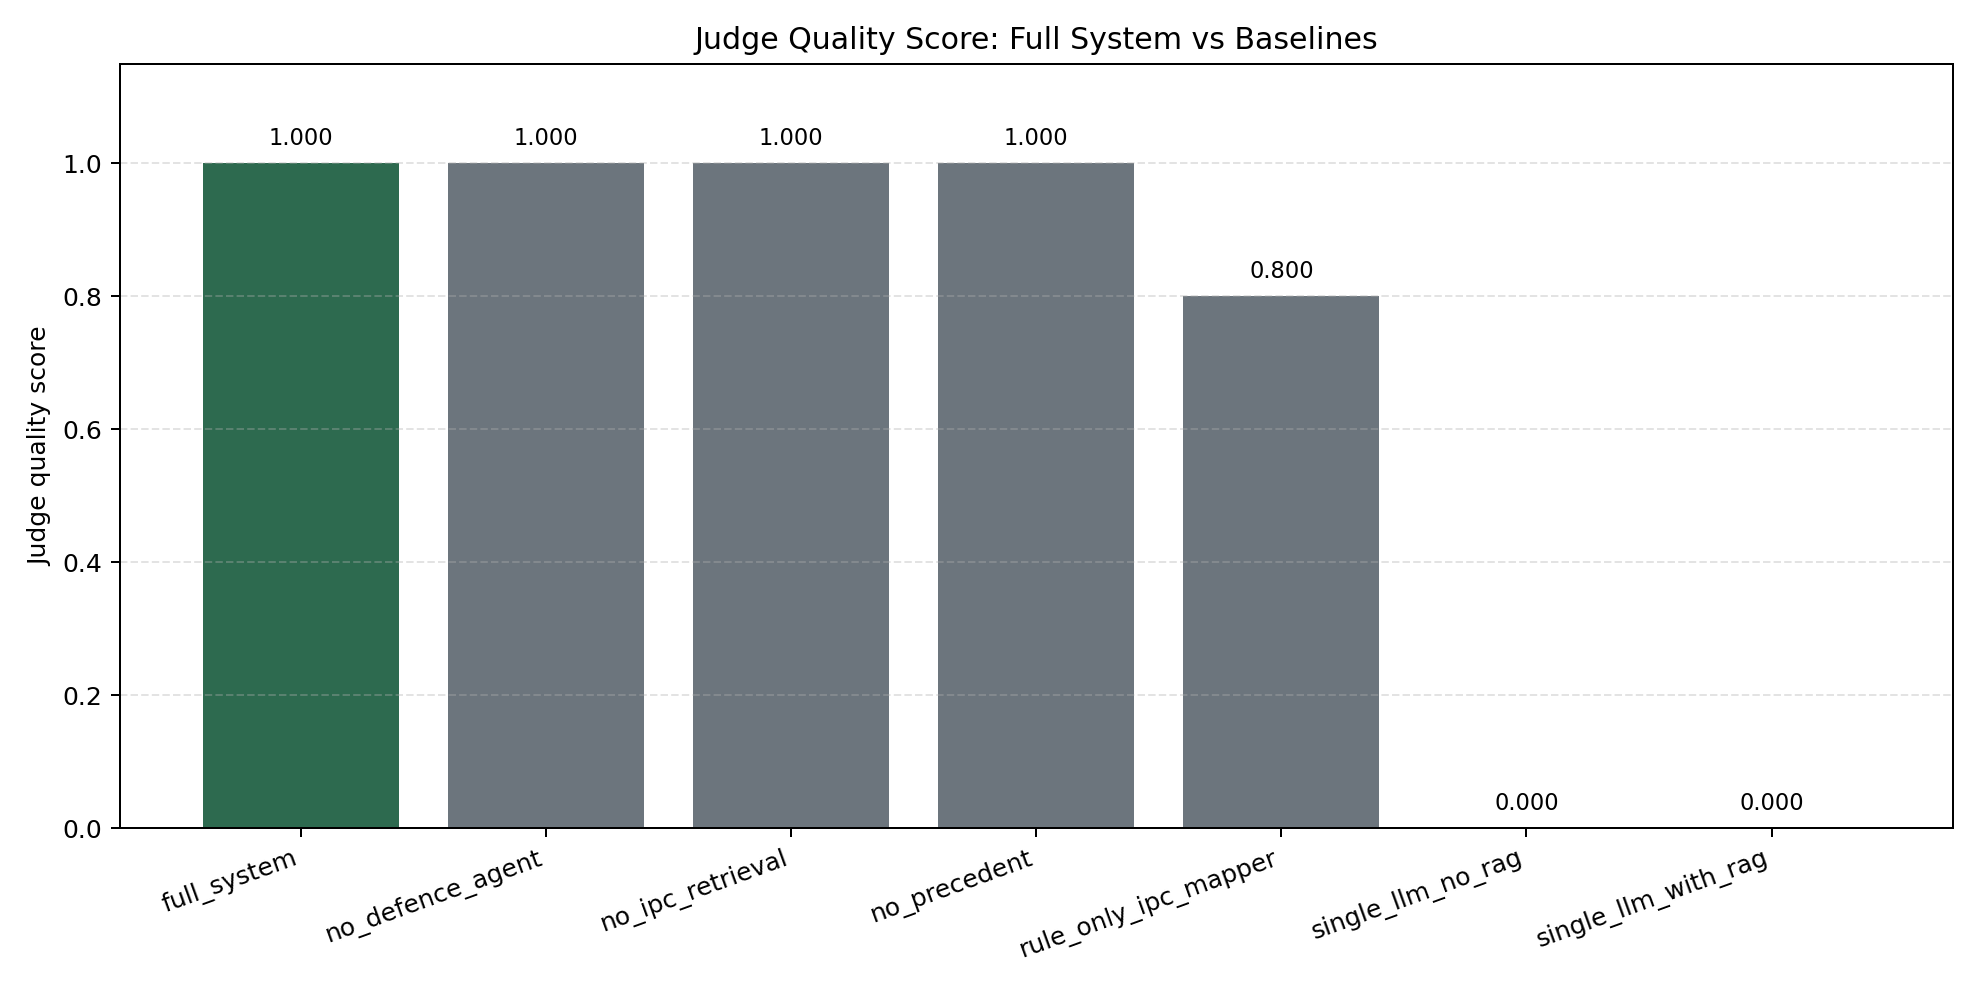
\includegraphics[width=\textwidth]{../experiments/reports/graphs_20cases/all_systems_judge_quality.png}}{\fbox{\parbox{0.95\columnwidth}{\centering\footnotesize Missing judge quality graph}}}
\end{minipage}
\hfill
\begin{minipage}[t]{0.32\columnwidth}
\centering
\IfFileExists{../experiments/reports/graphs_20cases/all_systems_defence_quality.png}{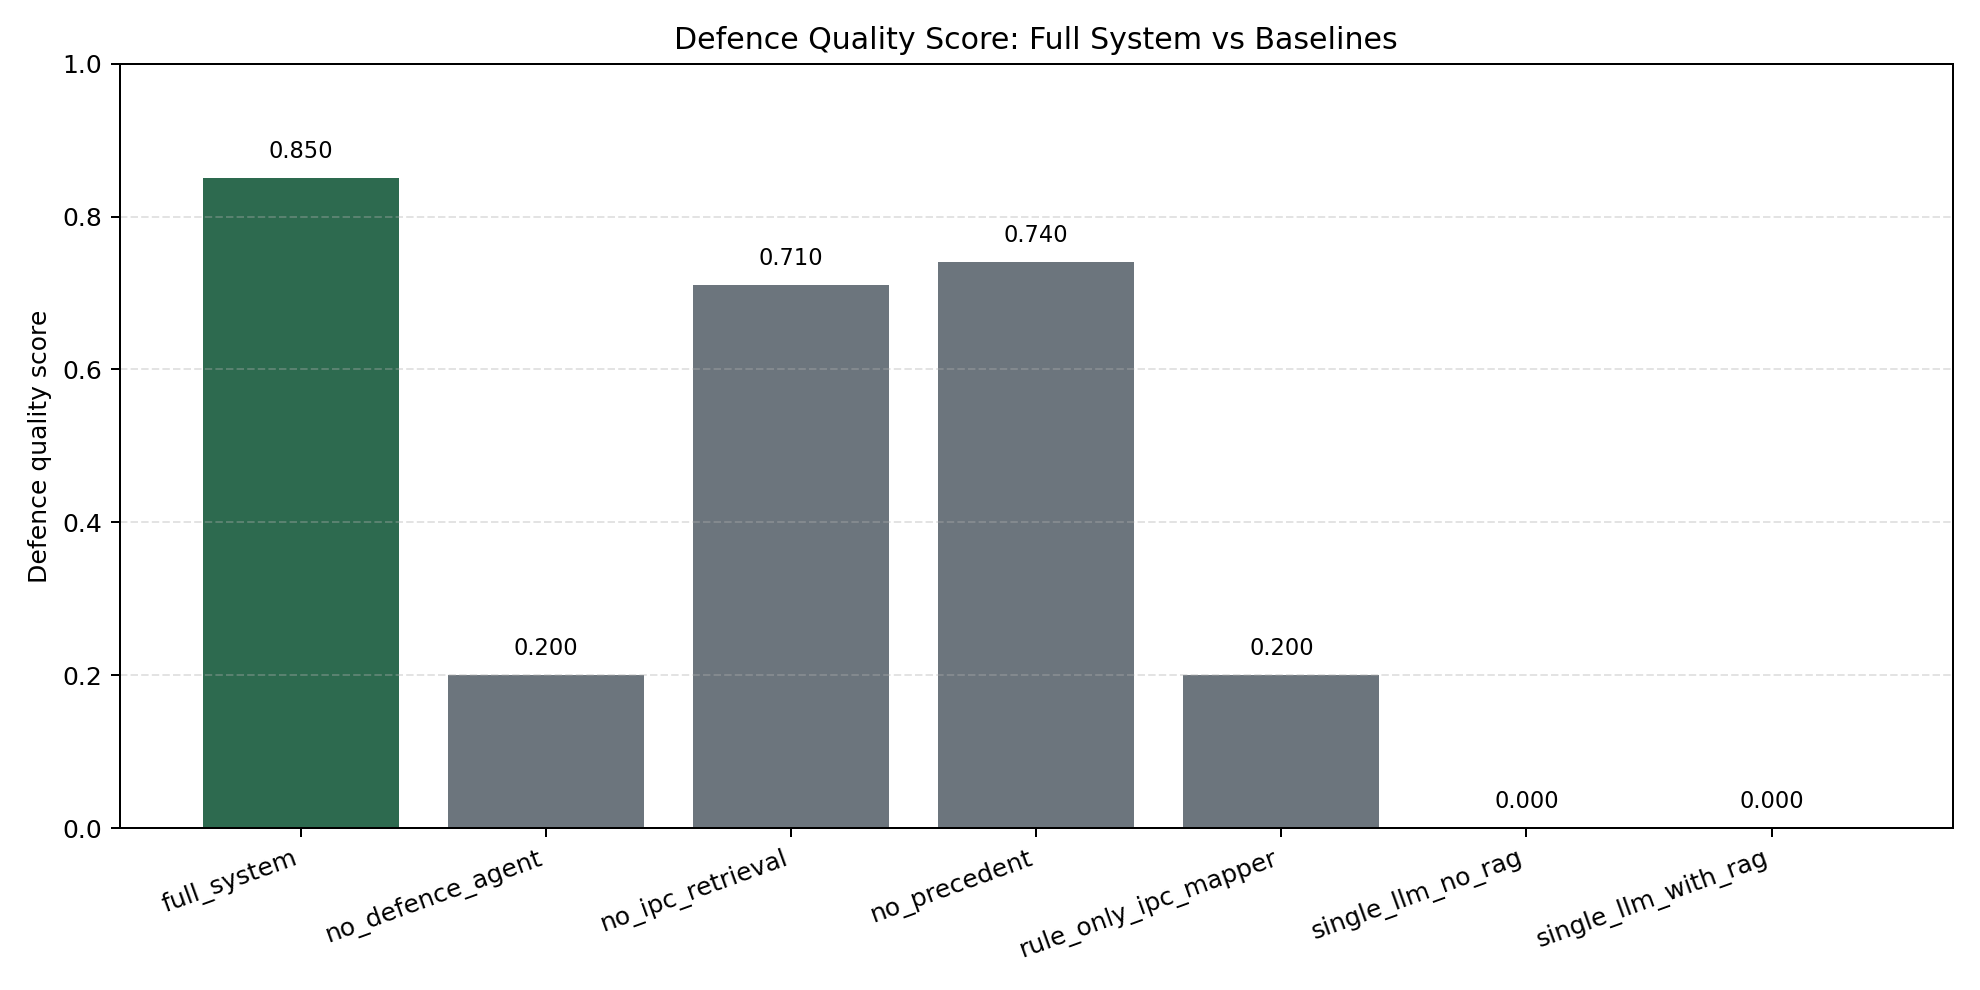
\includegraphics[width=\textwidth]{../experiments/reports/graphs_20cases/all_systems_defence_quality.png}}{\fbox{\parbox{0.95\columnwidth}{\centering\footnotesize Missing defence quality graph}}}
\end{minipage}
\hfill
\begin{minipage}[t]{0.32\columnwidth}
\centering
\IfFileExists{../experiments/reports/graphs_20cases/all_systems_judge_ipc_recall.png}{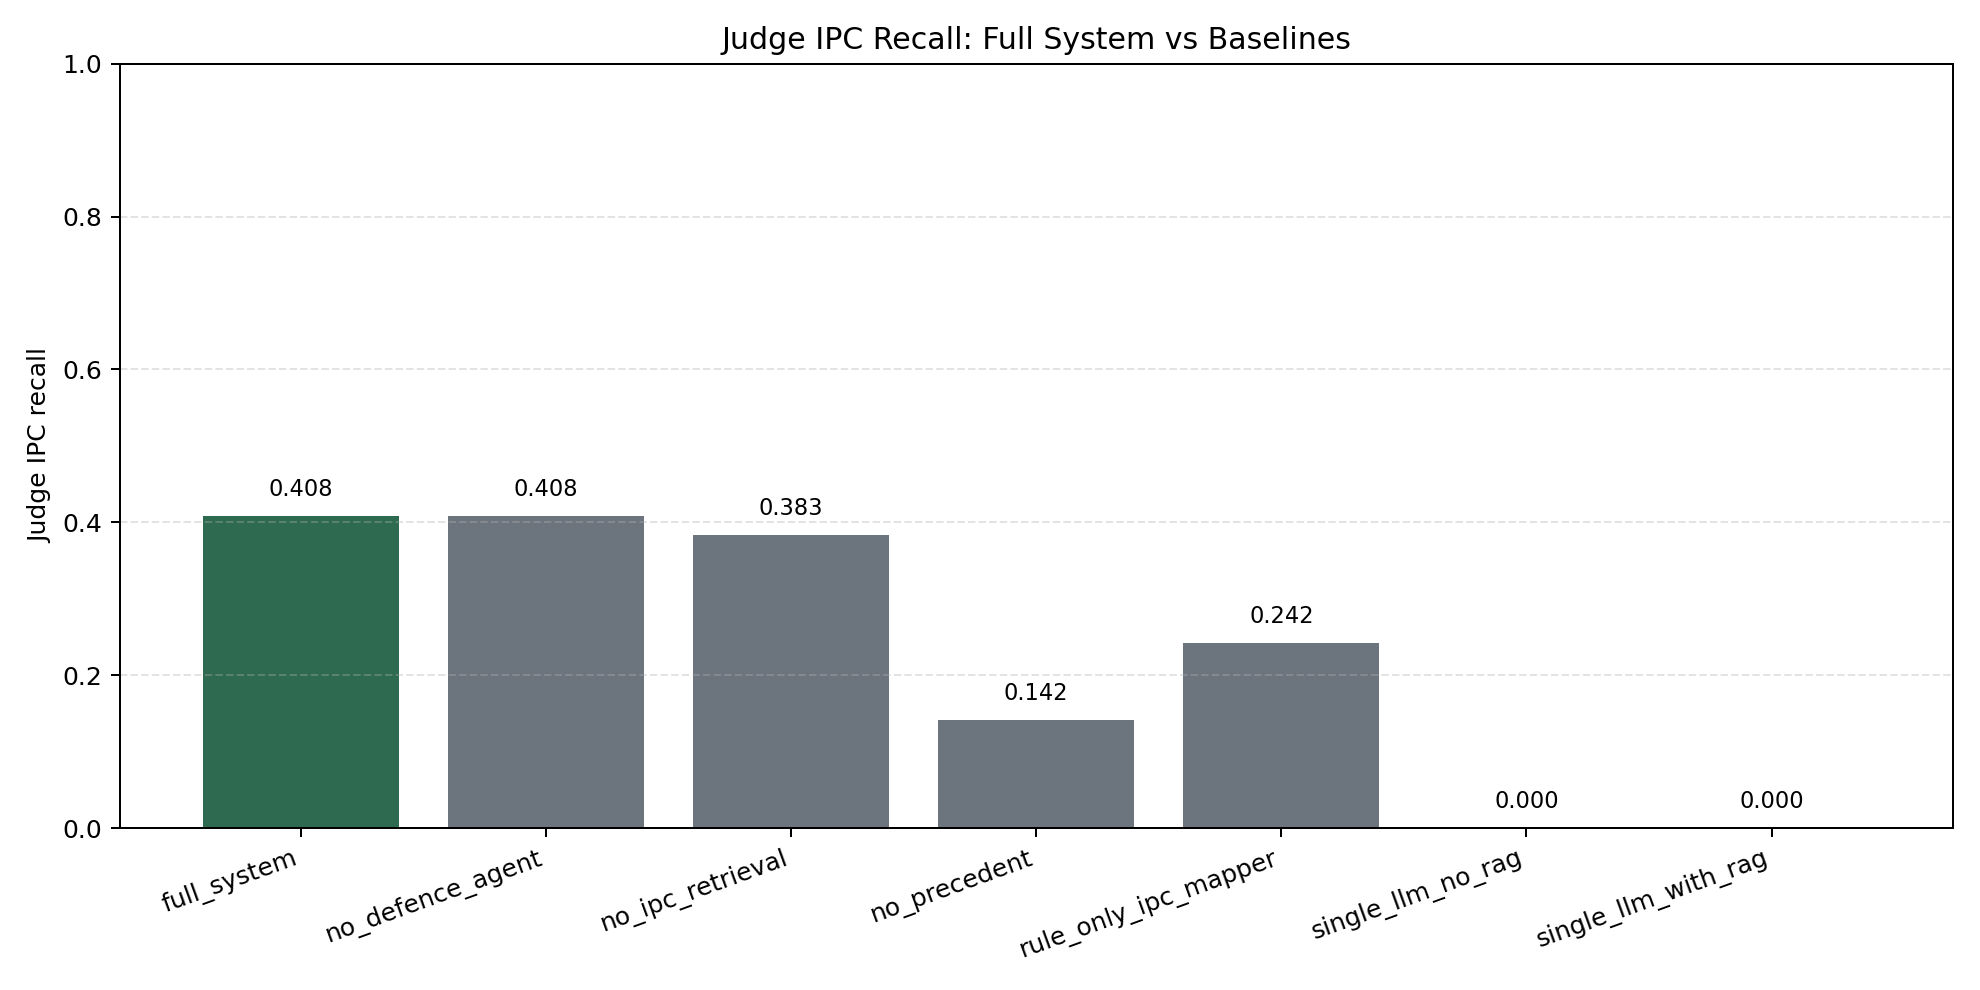
\includegraphics[width=\textwidth]{../experiments/reports/graphs_20cases/all_systems_judge_ipc_recall.png}}{\fbox{\parbox{0.95\columnwidth}{\centering\footnotesize Missing judge IPC recall graph}}}
\end{minipage}

\caption{Variant-wise quality comparison for judge quality, defence quality, and judge IPC recall.}
\label{fig:quality_graphs}
\end{figure}

\begin{figure}[!t]
\centering

\begin{minipage}[t]{0.48\columnwidth}
\centering
\IfFileExists{../experiments/reports/graphs_20cases/full_vs_no_defence_deltas.png}{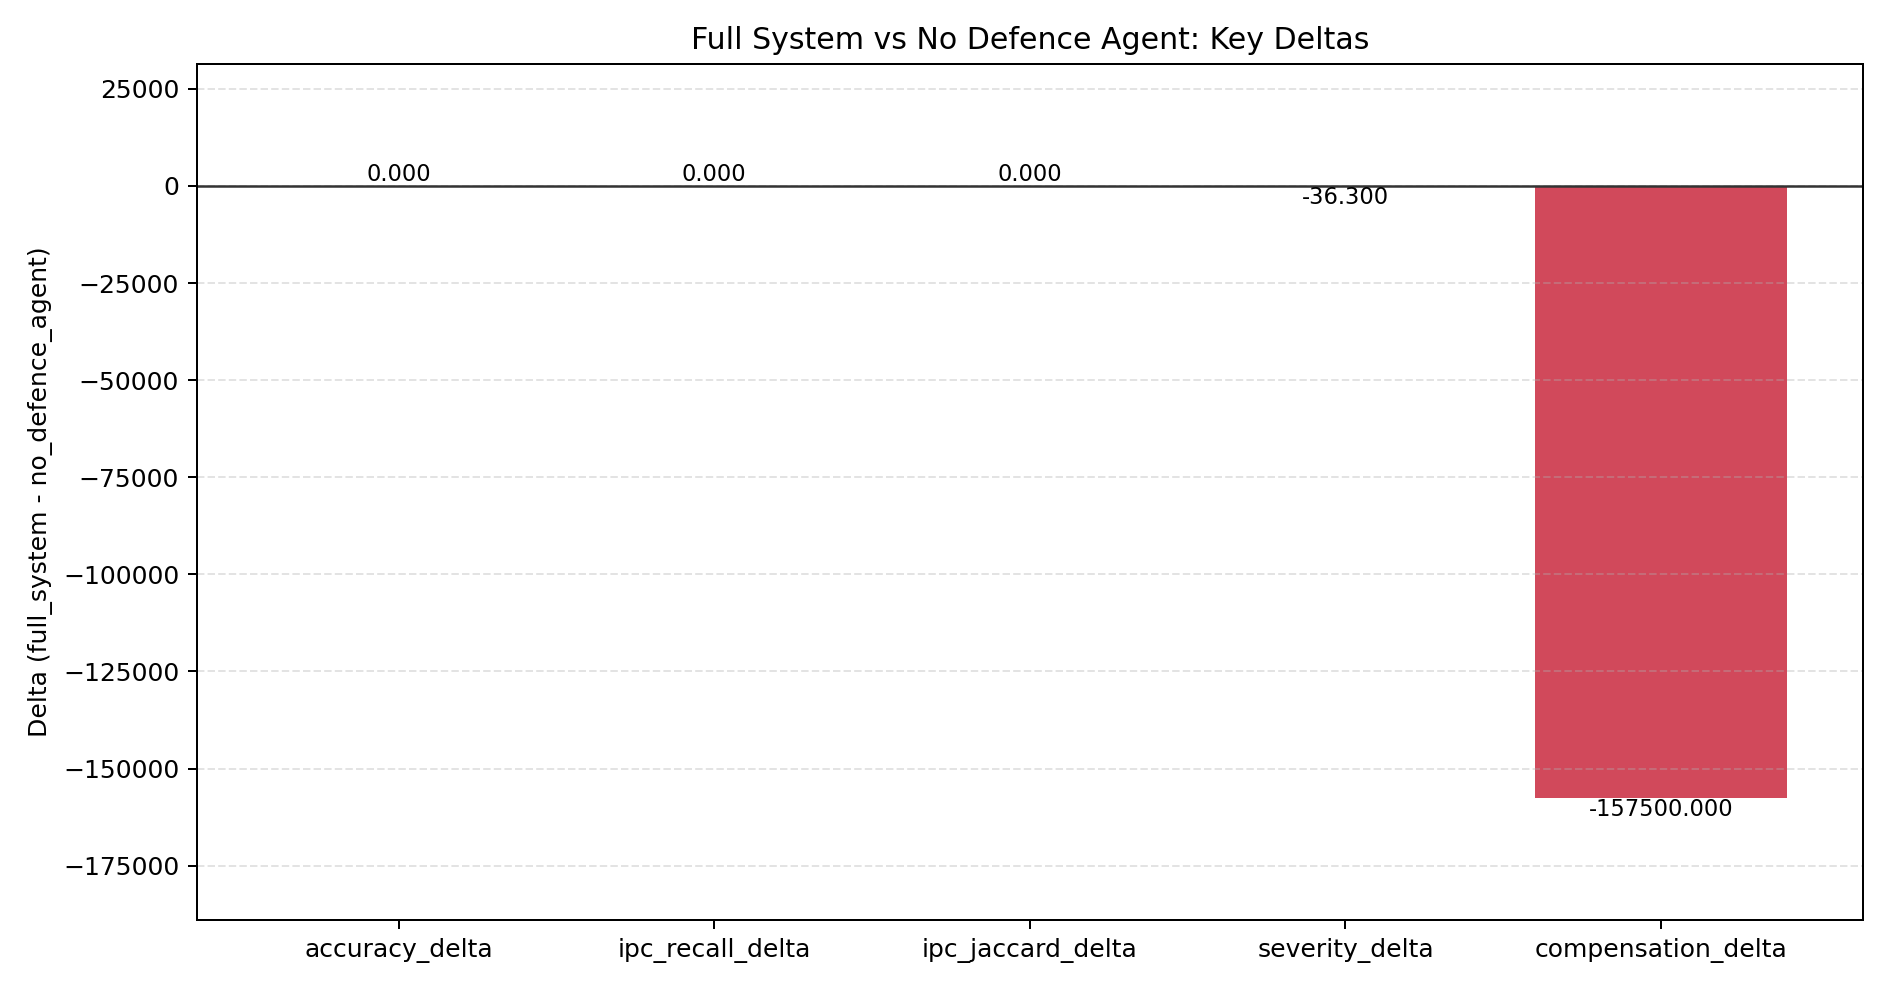
\includegraphics[width=\textwidth]{../experiments/reports/graphs_20cases/full_vs_no_defence_deltas.png}}{\fbox{\parbox{0.95\columnwidth}{\centering\footnotesize Missing full vs no-defence deltas graph}}}
\end{minipage}
\hfill
\begin{minipage}[t]{0.48\columnwidth}
\centering
\IfFileExists{../experiments/reports/graphs_20cases/full_vs_no_defence_severity_counts.png}{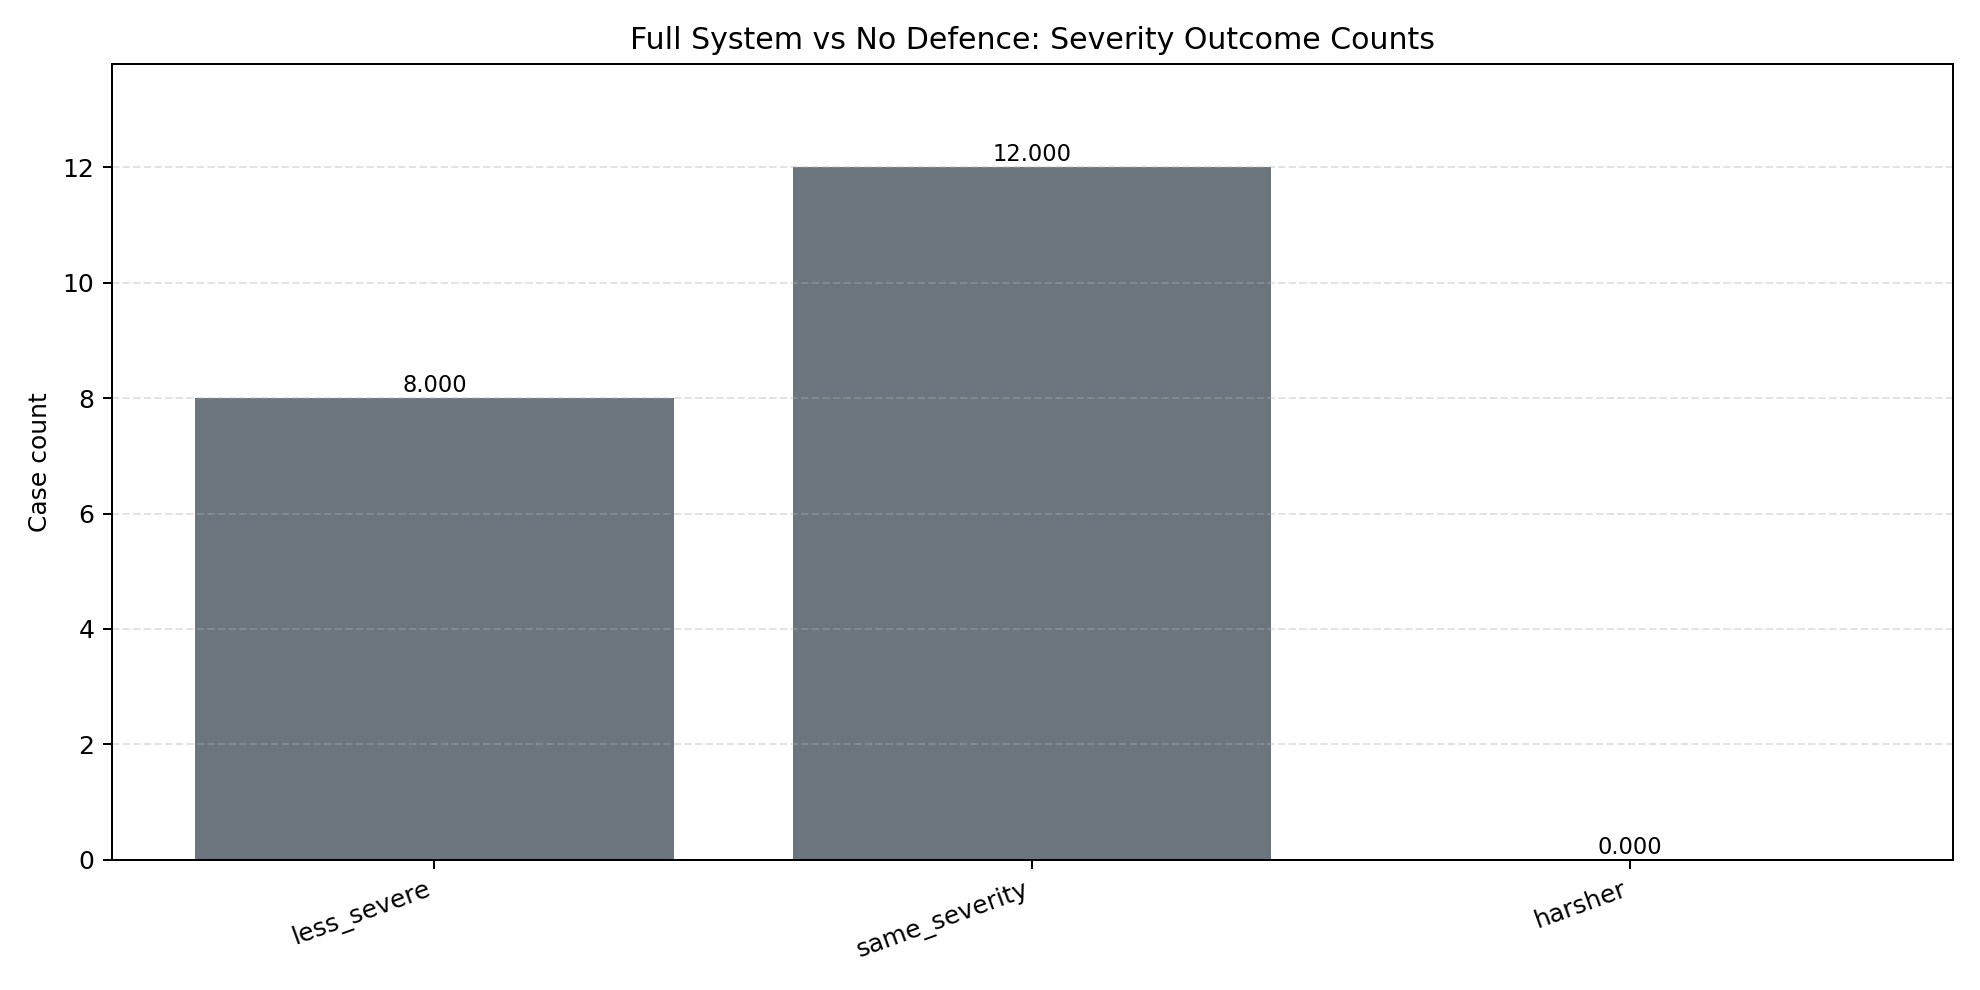
\includegraphics[width=\textwidth]{../experiments/reports/graphs_20cases/full_vs_no_defence_severity_counts.png}}{\fbox{\parbox{0.95\columnwidth}{\centering\footnotesize Missing severity count graph}}}
\end{minipage}

\caption{Ablation-focused graphs comparing \textit{full\_system} and \textit{no\_defence\_agent}.}
\label{fig:ablation_graphs}
\end{figure}

\FloatBarrier
\section{Error Analysis}
Three recurring error modes were observed:
\begin{itemize}
\item \textbf{Over-inclusive charging:} the model sometimes predicts supersets of applicable IPC sections, which inflates recall while reducing precision.
\item \textbf{Sentencing mismatch:} textual sentencing recommendations may be directionally correct but not exact enough for strict-match evaluation.
\item \textbf{Retrieval brittleness:} precedent retrieval quality is sensitive to chunk granularity and citation-style lexical mismatch.
\end{itemize}

\section{Limitations and Future Work}
Current experiments are limited by dataset size and API variability, and some baseline rows were excluded as invalid. Future work will focus on (i) larger and harder benchmark sets with richer fact patterns, (ii) calibrated confidence estimation for each predicted IPC section, (iii) citation-level faithfulness checks between generated claims and retrieved evidence, and (iv) domain-adapted rerankers for legal precedents.

\section{Conclusion}
This paper presented a multi-agent IPC reasoning system that combines hybrid legal retrieval with prosecutor-defence-judge role decomposition and judge-stage evidence isolation. The approach improves legal argument quality and transparency relative to simplified baselines, while revealing important open challenges in exact judgment matching and robust precedent retrieval. The system is practical as a legal education and decision-support scaffold, and provides a reproducible foundation for future research in accountable legal AI.

\section*{Acknowledgment}
This work was carried out as part of an academic project on legal AI for IPC case reasoning. The authors thank their mentors and peers for feedback on benchmark design and evaluation methodology.

\section*{References}

\begin{thebibliography}{00}
\bibitem{lewis2020rag} P. Lewis \textit{et al.}, ``Retrieval-augmented generation for knowledge-intensive NLP tasks,'' in \textit{Advances in Neural Information Processing Systems}, vol. 33, 2020, pp. 9459--9474.
\bibitem{thakur2021beir} N. Thakur \textit{et al.}, ``BEIR: A heterogeneous benchmark for zero-shot evaluation of information retrieval models,'' in \textit{Proc. NeurIPS Datasets and Benchmarks}, 2021.
\bibitem{autogen2023} Q. Wu \textit{et al.}, ``AutoGen: Enabling next-gen LLM applications via multi-agent conversation,'' 2023, arXiv:2308.08155.
\bibitem{chalkidis2019legalbert} I. Chalkidis, M. Fergadiotis, P. Malakasiotis, and I. Androutsopoulos, ``Large-scale multi-label text classification on EU legislation,'' in \textit{Proc. ACL}, 2019.
\bibitem{katz2017legal} D. M. Katz, M. J. Bommarito, and J. Blackman, ``A general approach for predicting the behavior of the Supreme Court of the United States,'' \textit{PLOS ONE}, vol. 12, no. 4, 2017.
\bibitem{ipc1860} Government of India, ``The Indian Penal Code, 1860,'' Legislative Department, Ministry of Law and Justice.
\bibitem{faiss2017} J. Johnson, M. Douze, and H. Jegou, ``Billion-scale similarity search with GPUs,'' 2017, arXiv:1702.08734.
\bibitem{bm25} S. Robertson and H. Zaragoza, ``The probabilistic relevance framework: BM25 and beyond,'' \textit{Foundations and Trends in Information Retrieval}, vol. 3, no. 4, pp. 333--389, 2009.
\end{thebibliography}

\end{document}
